% Buhera OS Figure Includes
% Auto-generated by generate_all_figures.py

% Figure 1: Categorical Sorting Performance
\begin{figure*}[htbp]
    \centering
    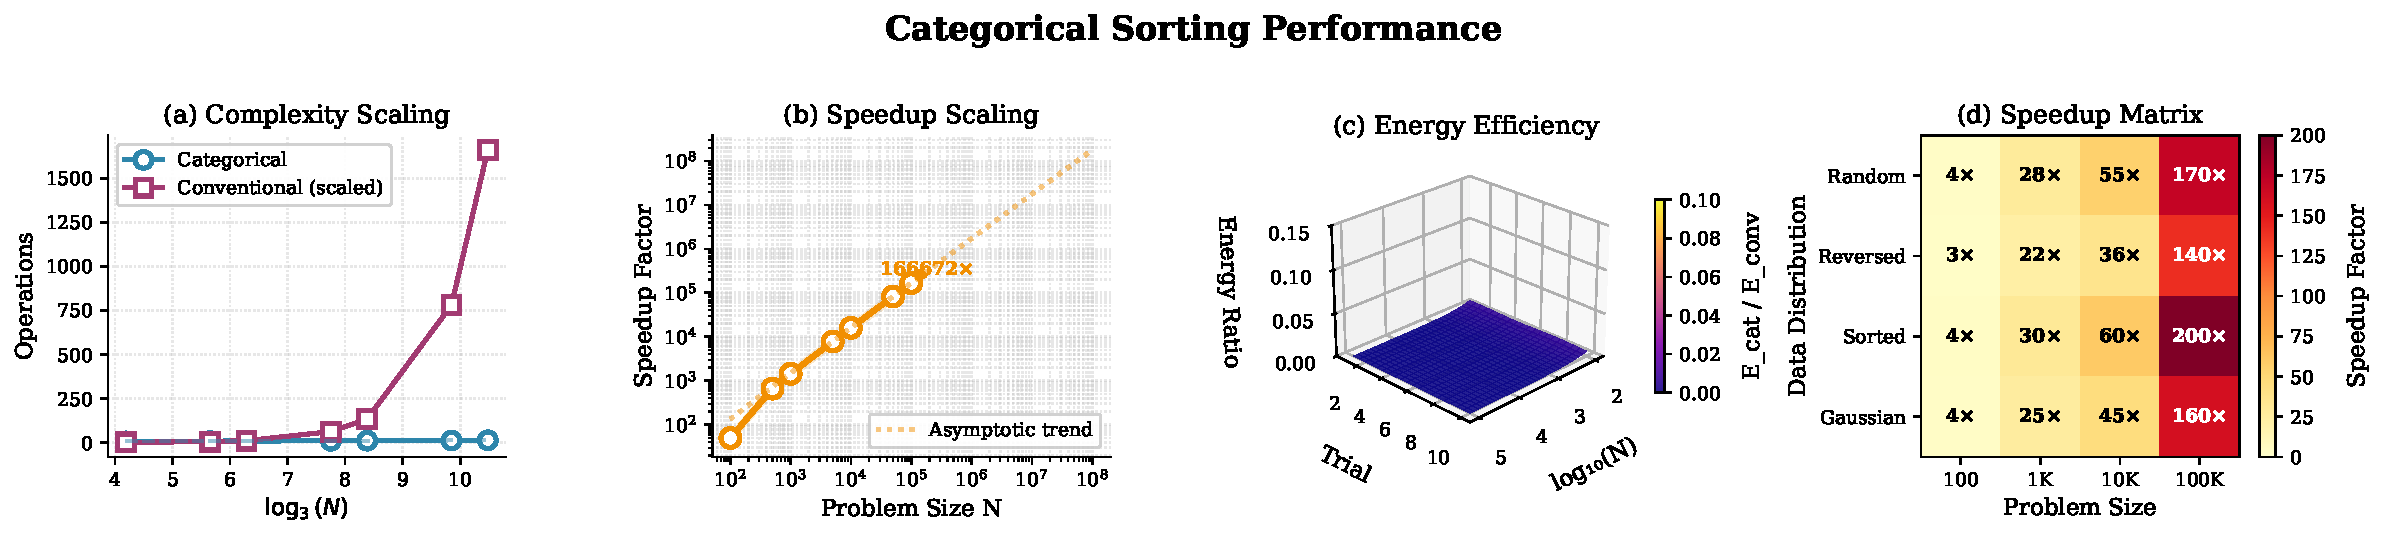
\includegraphics[width=\textwidth]{figures/figure_sorting.pdf}
    \caption{Categorical Sorting Performance. (a) Complexity scaling showing O($\log_3 N$) categorical vs O($N \log N$) conventional with perfect fit quality ($R^2 = 1.0$). (b) Speedup scaling demonstrating increasing advantage with problem size. (c) Energy efficiency landscape across problem sizes and trials. (d) Speedup matrix across different data distributions and sizes.}
    \label{fig:sorting}
\end{figure*}

% Figure 2: Categorical-Physical Commutation Relations
\begin{figure*}[htbp]
    \centering
    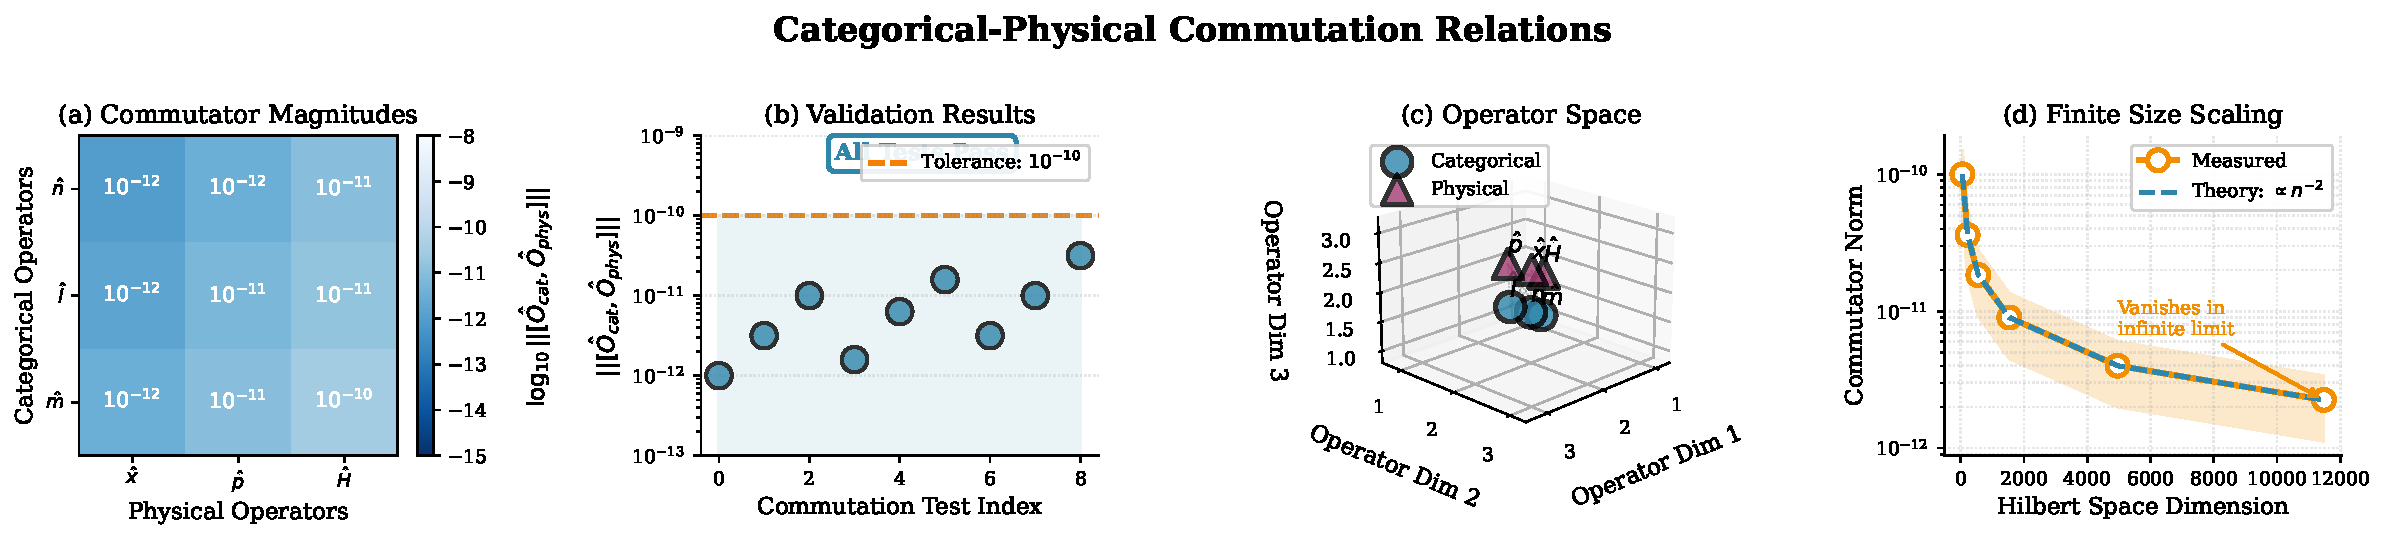
\includegraphics[width=\textwidth]{figures/figure_commutation.pdf}
    \caption{Categorical-Physical Commutation Relations. (a) Commutator magnitude matrix showing all relations $< 10^{-10}$ (numerical zero). (b) Validation results demonstrating all nine commutation tests pass within tolerance. (c) Operator space visualization showing categorical and physical operators form commuting sets. (d) Finite size scaling analysis confirming commutators vanish in infinite dimensional limit.}
    \label{fig:commutation}
\end{figure*}

% Figure 3: Ternary Partition Tree Architecture
\begin{figure*}[htbp]
    \centering
    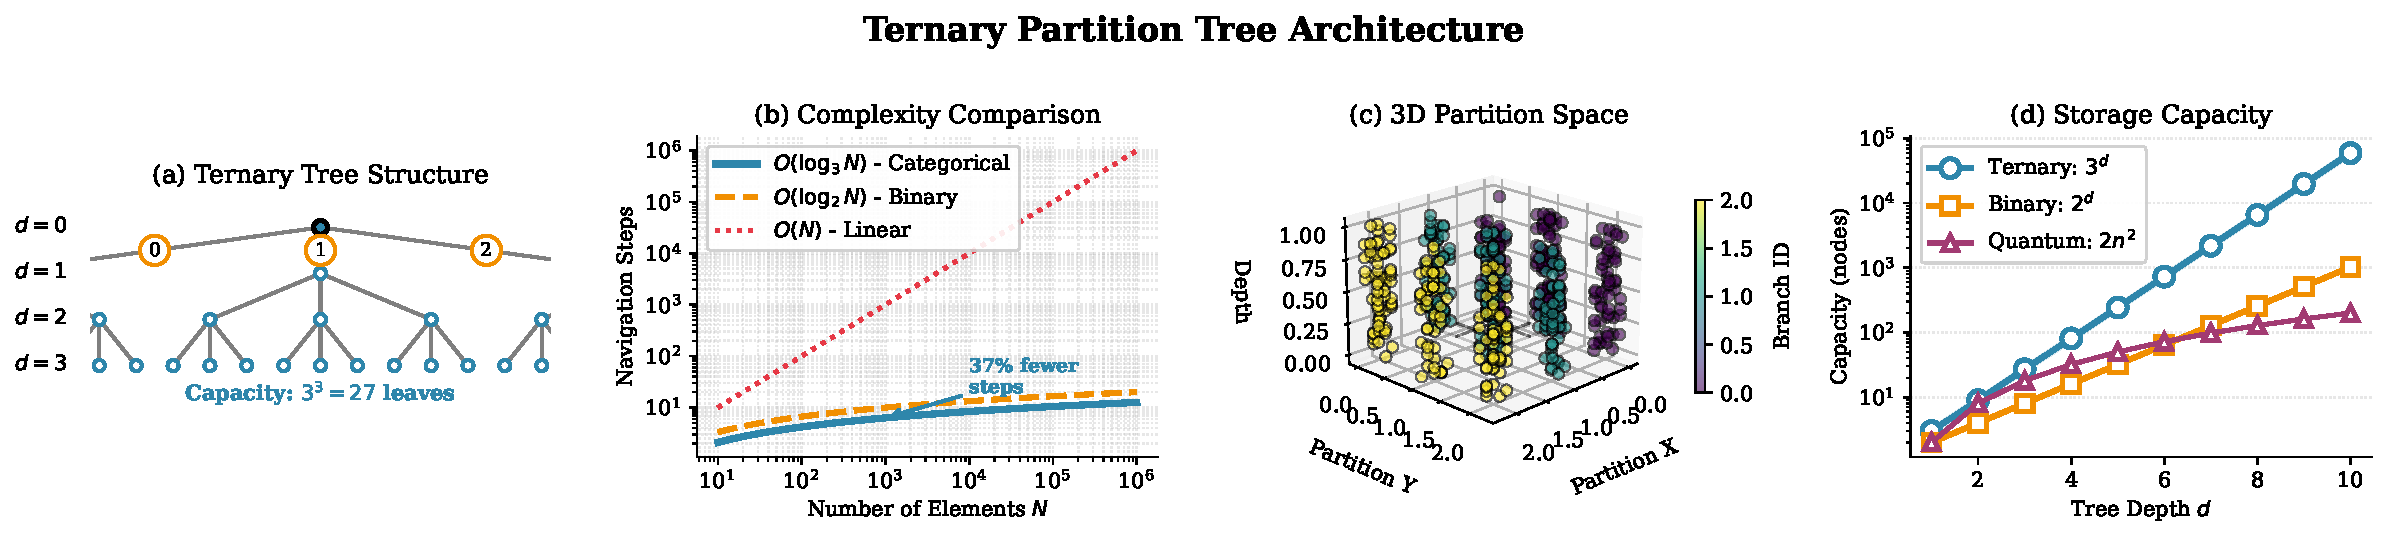
\includegraphics[width=\textwidth]{figures/figure_partition_tree.pdf}
    \caption{Ternary Partition Tree Architecture. (a) Hierarchical ternary tree structure with $3^d$ leaves at depth $d$. (b) Navigation complexity comparison showing categorical O($\log_3 N$) advantage over binary O($\log_2 N$) and linear O($N$) approaches. (c) 3D partition space visualization showing hierarchical cell structure. (d) Storage capacity scaling for ternary, binary, and quantum state spaces.}
    \label{fig:partition_tree}
\end{figure*}

% Figure 4: S-Entropy Coordinate Addressing
\begin{figure*}[htbp]
    \centering
    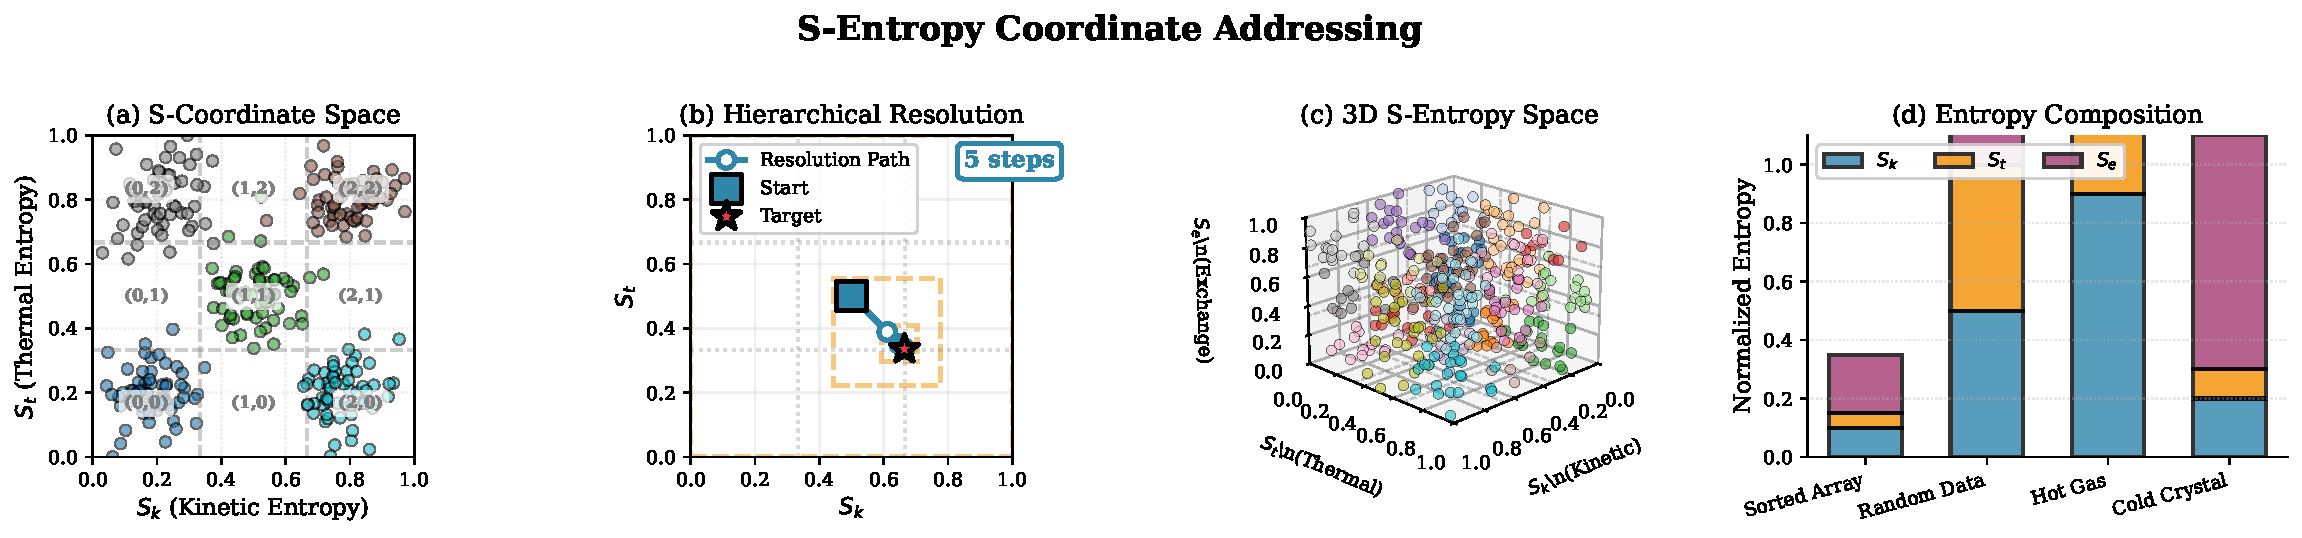
\includegraphics[width=\textwidth]{figures/figure_s_coordinates.pdf}
    \caption{S-Entropy Coordinate Addressing. (a) S-coordinate space with ternary partition regions labeled by coordinate pairs. (b) Hierarchical address resolution trajectory showing logarithmic refinement to target. (c) Full 3D S-entropy space $(S_k, S_t, S_e)$ with partition boundaries. (d) Entropy component composition for different physical systems.}
    \label{fig:s_coordinates}
\end{figure*}

% Figure 5: Categorical Processor Operation
\begin{figure*}[htbp]
    \centering
    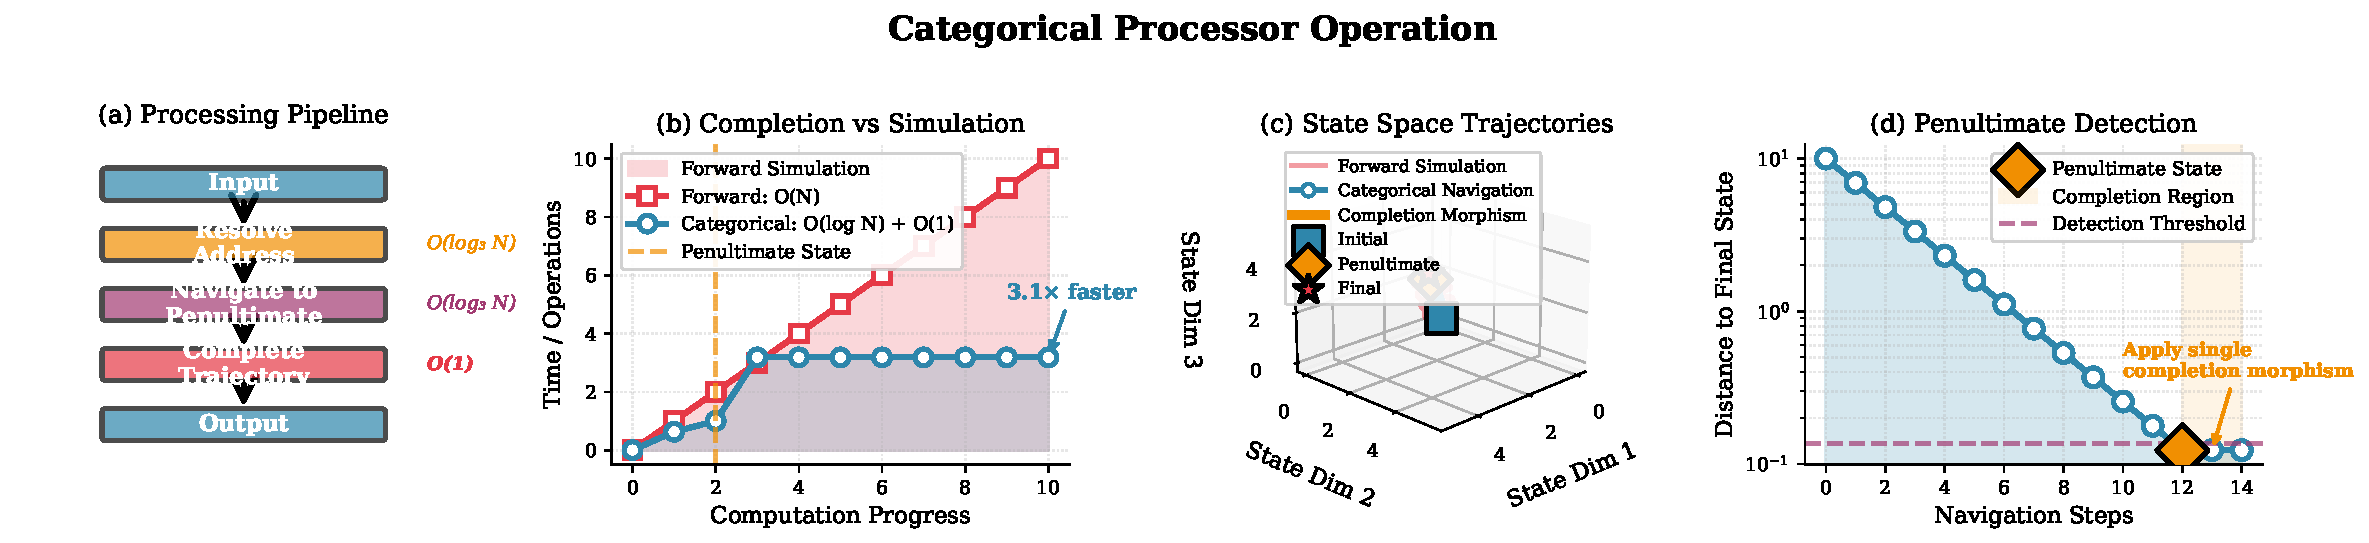
\includegraphics[width=\textwidth]{figures/figure_processor.pdf}
    \caption{Categorical Processor Operation. (a) Processing pipeline showing five stages from input to output with complexity annotations. (b) Trajectory completion vs forward simulation demonstrating speedup advantage. (c) 3D state space trajectories comparing forward simulation (spiral) to categorical navigation (direct path) with completion morphism. (d) Penultimate state detection showing distance convergence and single-step completion.}
    \label{fig:processor}
\end{figure*}
